% =====================================================================
%  Aprendizaje No Supervisado — Sesión 4: Modelos de mezclas gaussianas (GMM)
%  Unidad 1: Algoritmos de agrupamiento
%  Compilar con: latexmk -pdf Sesion4-GMM.tex
%  Figuras: python3 figuras/generar_figuras.py
%  El laboratorio está en Laboratorio.tex (se incluye al final con \input)
% =====================================================================
\documentclass[aspectratio=169,11pt]{beamer}

\usepackage[utf8]{inputenc}
\usepackage[T1]{fontenc}
\usepackage[spanish,es-noshorthands,es-nodecimaldot]{babel}
\usepackage{amsmath,amssymb,bm}
\usepackage{booktabs,array}
\usepackage{listings}
\usepackage{tikz}
\usetikzlibrary{positioning,arrows.meta}
\graphicspath{{figuras/}}
\tikzset{caja/.style={draw=azul,fill=azul!10,rounded corners,align=center,font=\small,
  minimum height=9mm}}

% ---------- Tema (común a las presentaciones del curso) ----------
\usetheme{Madrid}
\usefonttheme{professionalfonts}
\definecolor{marino}{HTML}{1F3864}
\definecolor{azul}{HTML}{2E75B6}
\definecolor{naranja}{HTML}{E07B22}
\definecolor{verde}{HTML}{5B9A3C}
\definecolor{fondocod}{HTML}{F4F6F9}
\setbeamercolor{palette primary}{bg=marino,fg=white}
\setbeamercolor{palette secondary}{bg=azul,fg=white}
\setbeamercolor{palette tertiary}{bg=marino,fg=white}
\setbeamercolor{frametitle}{bg=marino,fg=white}
\setbeamercolor{title}{bg=marino,fg=white}
\setbeamercolor{structure}{fg=azul}
\setbeamercolor{block title}{bg=azul,fg=white}
\setbeamercolor{block body}{bg=azul!8}
\setbeamercolor{block title alerted}{bg=naranja,fg=white}
\setbeamercolor{block body alerted}{bg=naranja!10}
\setbeamercolor{block title example}{bg=verde,fg=white}
\setbeamercolor{block body example}{bg=verde!10}
\setbeamercolor{alerted text}{fg=naranja}
\setbeamertemplate{navigation symbols}{}
\setbeamertemplate{itemize items}[circle]
\setbeamertemplate{blocks}[rounded][shadow=false]

\AtBeginSection[]{
  \begin{frame}
    \vfill\centering
    \begin{beamercolorbox}[sep=12pt,center,rounded=true]{title}
      \usebeamerfont{title}\insertsectionhead
    \end{beamercolorbox}
    \vfill
  \end{frame}
}

\lstdefinestyle{py}{
  language=Python, basicstyle=\ttfamily\scriptsize,
  keywordstyle=\color{marino}\bfseries, commentstyle=\color{gray}\itshape,
  stringstyle=\color{naranja}, backgroundcolor=\color{fondocod},
  frame=single, rulecolor=\color{azul!40}, showstringspaces=false,
  columns=fullflexible, breaklines=true, xleftmargin=4pt, xrightmargin=4pt
}
\lstset{style=py}

\newcommand{\R}{\mathbb{R}}
\newcommand{\x}{\bm{x}}
\newcommand{\muv}{\bm{\mu}}
\newcommand{\Sig}{\bm{\Sigma}}
\newcommand{\N}{\mathcal{N}}

\title[Sesión 4: Mezclas gaussianas]{Sesión 4: Modelos de mezclas gaussianas (GMM)}
\subtitle{Aprendizaje No Supervisado --- Unidad 1: Algoritmos de agrupamiento}
\author[A. Espinosa Romero]{Arturo Espinosa Romero}
\institute[FMAT]{Maestría en Inteligencia Artificial \\ Facultad de Matemáticas}
\date{Sesión 4}

% =====================================================================
\begin{document}

\begin{frame}
  \titlepage
\end{frame}

\begin{frame}{Agenda de la sesión}
  \begin{columns}[T]
    \column{0.55\textwidth}
    \begin{enumerate}
      \item Agrupamiento probabilístico y asignaciones suaves
      \item El algoritmo de esperanza-maximización (EM)
      \item Tipos de matriz de covarianza
      \item Selección de modelo con BIC y AIC
      \item Laboratorio: GMM y k-medias en Iris
    \end{enumerate}
    \column{0.4\textwidth}
    \begin{block}{Al terminar podrás}
      \begin{itemize}
        \item Describir un agrupamiento como un modelo generativo
        \item Explicar los pasos E y M
        \item Elegir el tipo de covarianza
        \item Elegir el número de componentes con BIC
      \end{itemize}
    \end{block}
  \end{columns}
\end{frame}

% =====================================================================
\section{Agrupamiento probabilístico}
% =====================================================================

\begin{frame}{Problema detonador: grupos alargados}
  \centering
  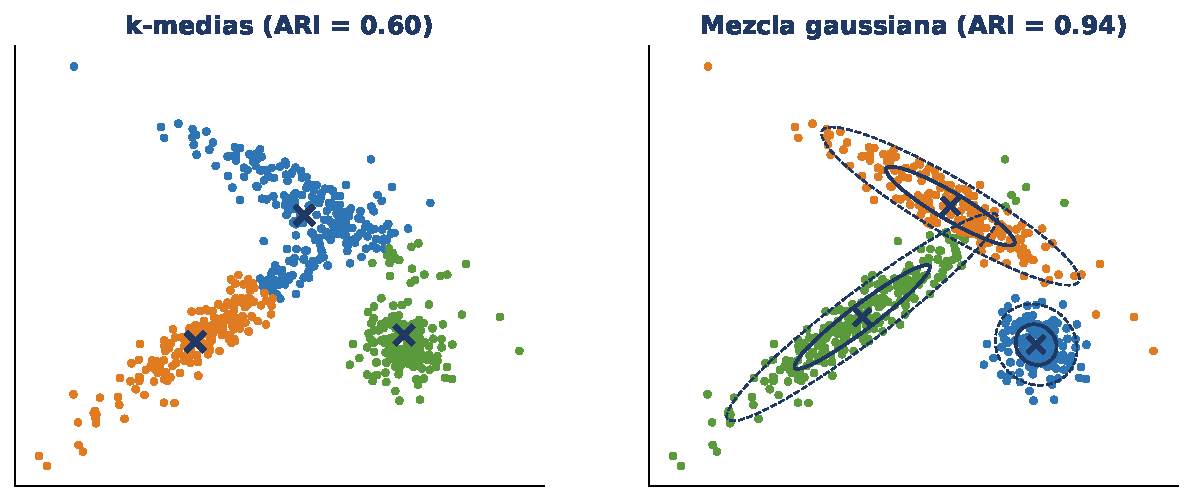
\includegraphics[width=0.78\textwidth]{detonador}
  \begin{itemize}
    \item Tres grupos de forma, tamaño y orientación distintos (600 puntos).
    \item k-medias parte los grupos alargados: asigna cada punto al centro más cercano,
          y eso equivale a suponer grupos \alert{esféricos} del mismo tamaño.
    \item Una mezcla de gaussianas aprende la forma de cada grupo (las elipses).
  \end{itemize}
\end{frame}

\begin{frame}{Lo que k-medias supone sin decirlo}
  \begin{columns}[T]
    \column{0.5\textwidth}
    \begin{block}{Supuestos implícitos de k-medias}
      \begin{itemize}
        \item Grupos esféricos: sólo cuenta la distancia euclidiana al centro.
        \item Grupos de tamaño (varianza) parecido.
        \item Asignación \textbf{dura}: cada punto pertenece a un solo grupo,
              aunque esté en la frontera.
      \end{itemize}
    \end{block}
    \column{0.46\textwidth}
    \begin{exampleblock}{Lo que agrega una mezcla gaussiana}
      \begin{itemize}
        \item Cada grupo tiene su propia covarianza: elipses de cualquier orientación.
        \item Cada grupo tiene su propio peso: grupos de tamaños distintos.
        \item Asignación \textbf{suave}: la probabilidad de pertenecer a cada grupo.
        \item Un modelo de densidad $p(\x)$: sirve también para detectar anomalías (Unidad 3).
      \end{itemize}
    \end{exampleblock}
  \end{columns}
\end{frame}

\begin{frame}{La gaussiana multivariada}
  \[
    \N(\x \mid \muv, \Sig) = \frac{1}{(2\pi)^{d/2}\,|\Sig|^{1/2}}
    \exp\!\Big(-\tfrac12 (\x-\muv)^\top \Sig^{-1} (\x-\muv)\Big)
  \]
  \centering
  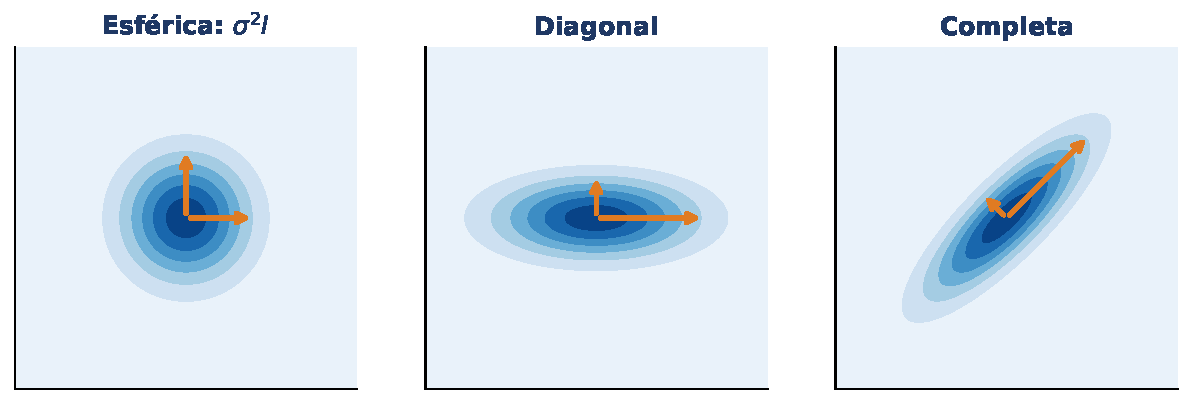
\includegraphics[width=0.72\textwidth]{gaussianas_2d}
  \begin{itemize}
    \item Las curvas de nivel son elipses. Los ejes son los vectores propios de $\Sig$
          y su largo es proporcional a la raíz de los valores propios (flechas).
    \item $(\x-\muv)^\top \Sig^{-1} (\x-\muv)$ es la \textbf{distancia de Mahalanobis} al cuadrado.
  \end{itemize}
\end{frame}

\begin{frame}{El modelo de mezcla: cómo se generan los datos}
  \begin{columns}[c]
    \column{0.55\textwidth}
    Cada punto se genera en dos pasos:
    \begin{enumerate}
      \item Se elige un componente $z \in \{1,\dots,K\}$ con probabilidad $\pi_k$.
      \item Se genera $\x \sim \N(\muv_z, \Sig_z)$.
    \end{enumerate}
    \vspace{4pt}
    Al no observar $z$, la densidad de $\x$ es
    \[
      p(\x) = \sum_{k=1}^{K} \pi_k\, \N(\x \mid \muv_k, \Sig_k),
    \]
    con $\pi_k \ge 0$ y $\sum_k \pi_k = 1$.
    Parámetros: $\theta = \{\pi_k, \muv_k, \Sig_k\}_{k=1}^K$.
    \column{0.4\textwidth}
    \centering
    \begin{tikzpicture}[node distance=8mm, >={Stealth[length=2.5mm]}]
      \node[caja] (pi) {$\pi$};
      \node[caja, below=of pi, fill=naranja!15, draw=naranja] (z) {$z_i$\\{\scriptsize oculta}};
      \node[caja, below=of z, fill=azul!30] (x) {$\x_i$\\{\scriptsize observada}};
      \node[caja, right=6mm of x] (th) {$\muv_k, \Sig_k$};
      \draw[->] (pi) -- (z);
      \draw[->] (z) -- (x);
      \draw[->] (th) -- (x);
    \end{tikzpicture}
  \end{columns}
  \vspace{4pt}
  \begin{block}{Agrupar = inferir la variable oculta}
    El grupo de un punto es el componente $z_i$ que probablemente lo generó.
  \end{block}
\end{frame}

\begin{frame}{Asignaciones suaves: la responsabilidad}
  Por la regla de Bayes, la probabilidad de que el componente $k$ haya generado $\x_i$ es
  \[
    \gamma_{ik} = P(z_i = k \mid \x_i)
    = \frac{\pi_k\, \N(\x_i \mid \muv_k, \Sig_k)}{\sum_{j=1}^{K} \pi_j\, \N(\x_i \mid \muv_j, \Sig_j)} ,
    \qquad \sum_k \gamma_{ik} = 1 .
  \]
  \begin{itemize}
    \item $\gamma_{ik}$ es la \alert{responsabilidad} del componente $k$ sobre el punto $i$.
    \item Asignación suave: el vector $(\gamma_{i1},\dots,\gamma_{iK})$.
    \item Asignación dura (si se necesita): $\hat z_i = \arg\max_k \gamma_{ik}$.
    \item Un punto con $\max_k \gamma_{ik}$ cercano a $1/K$ está en una frontera:
          el modelo nos dice que \textbf{no está seguro}.
  \end{itemize}
\end{frame}

\begin{frame}{Ejemplo resuelto en una dimensión}
  \begin{columns}[c]
    \column{0.52\textwidth}
    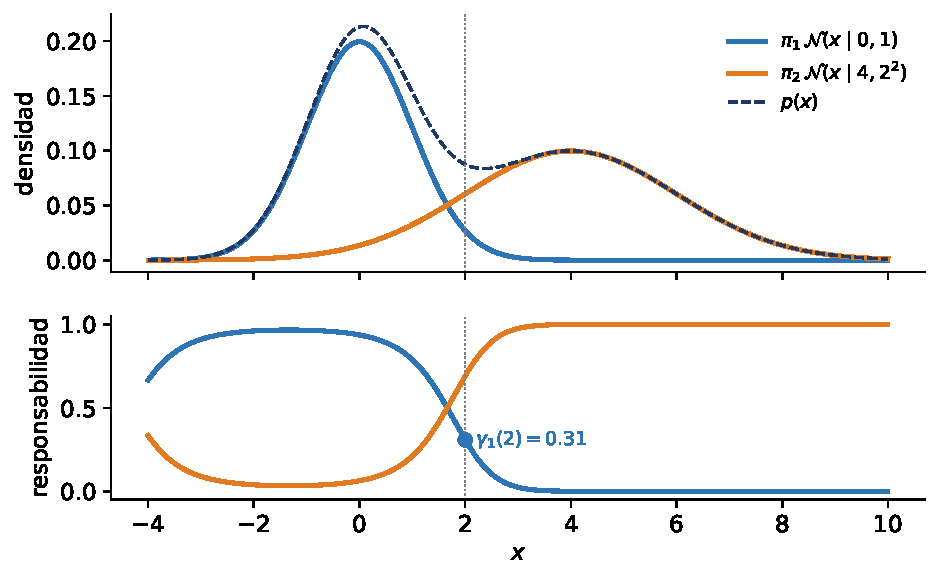
\includegraphics[width=\textwidth]{asignacion_suave}
    \column{0.46\textwidth}
    \small
    $\pi_1=\pi_2=0.5$, \ $\N(0, 1)$ y $\N(4, 2^2)$. En $x=2$:
    \begin{align*}
      \pi_1\,\N(2\mid 0,1)   &= 0.5 \times 0.0540 = 0.0270\\
      \pi_2\,\N(2\mid 4,2^2) &= 0.5 \times 0.1210 = 0.0605\\
      \gamma_1(2) &= \frac{0.0270}{0.0270+0.0605} = 0.31
    \end{align*}
    \begin{itemize}
      \item $x=2$ está a la misma distancia de ambas medias, pero el componente ancho es
            más responsable: 0.69 contra 0.31.
      \item k-medias lo asignaría a cualquiera de los dos (empate).
      \item Lejos a la izquierda vuelve a crecer la responsabilidad del componente ancho:
            su densidad decae más despacio.
    \end{itemize}
  \end{columns}
\end{frame}

% =====================================================================
\section{El algoritmo de esperanza-maximización (EM)}
% =====================================================================

\begin{frame}{Máxima verosimilitud con variables ocultas}
  Queremos los parámetros que maximizan la log-verosimilitud de los datos:
  \[
    \ell(\theta) = \sum_{i=1}^{n} \log \sum_{k=1}^{K} \pi_k\, \N(\x_i \mid \muv_k, \Sig_k).
  \]
  \begin{itemize}
    \item El logaritmo de una \textbf{suma} no se simplifica: igualar el gradiente a cero no
          tiene solución cerrada.
    \item Si conociéramos $z_i$, el problema sería fácil: para cada grupo, la media y la
          covarianza muestrales de sus puntos, y $\pi_k$ la proporción de puntos.
    \item No conocemos $z_i$, pero podemos calcular su probabilidad $\gamma_{ik}$ si conocemos $\theta$.
  \end{itemize}
  \vspace{4pt}
  \begin{block}{Idea de EM}
    Alternar: con $\theta$ fijo, estimar las $z_i$ (paso E); con esas estimaciones,
    reestimar $\theta$ (paso M).
  \end{block}
\end{frame}

\begin{frame}{Los dos pasos}
  \begin{columns}[T]
    \column{0.47\textwidth}
    \begin{block}{Paso E (esperanza)}
      Con los parámetros actuales, calcular las responsabilidades:
      \[
        \gamma_{ik} \leftarrow \frac{\pi_k\, \N(\x_i \mid \muv_k, \Sig_k)}{\sum_{j} \pi_j\, \N(\x_i \mid \muv_j, \Sig_j)}
      \]
    \end{block}
    \column{0.5\textwidth}
    \begin{block}{Paso M (maximización)}
      Con $N_k = \sum_i \gamma_{ik}$ (puntos ``efectivos'' del grupo $k$):
      \begin{align*}
        \pi_k  &\leftarrow N_k / n\\
        \muv_k &\leftarrow \tfrac{1}{N_k} \textstyle\sum_i \gamma_{ik}\, \x_i\\
        \Sig_k &\leftarrow \tfrac{1}{N_k} \textstyle\sum_i \gamma_{ik}\, (\x_i-\muv_k)(\x_i-\muv_k)^\top
      \end{align*}
    \end{block}
  \end{columns}
  \vspace{6pt}
  \begin{itemize}
    \item El paso M es el cálculo ``fácil'' con conteos fraccionarios: cada punto cuenta
          $\gamma_{ik}$ en el grupo $k$.
    \item Se repite hasta que $\ell(\theta)$ deja de crecer (tolerancia \texttt{tol}).
  \end{itemize}
\end{frame}

\begin{frame}{EM en acción}
  \centering
  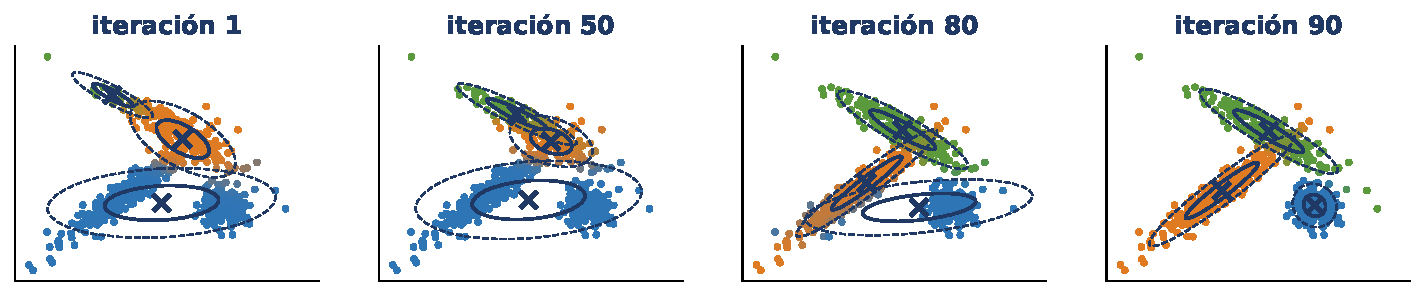
\includegraphics[width=0.95\textwidth]{em_iteraciones}
  \begin{columns}[c]
    \column{0.42\textwidth}
    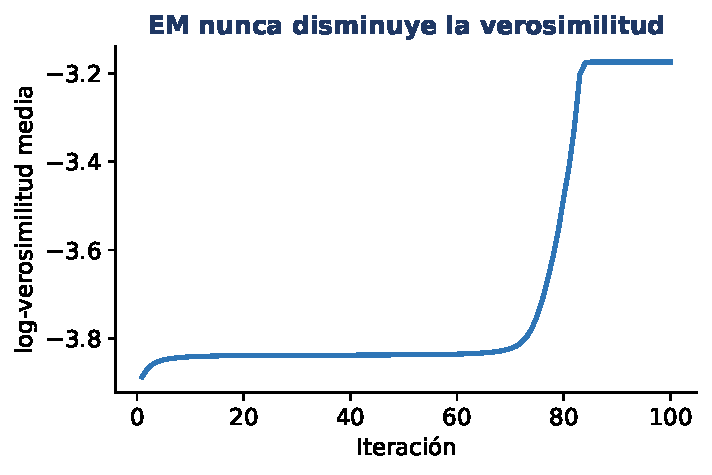
\includegraphics[width=\textwidth]{em_verosimilitud}
    \column{0.55\textwidth}
    \small
    \begin{itemize}
      \item Inicio con medias tomadas al azar de los datos; el color mezcla las responsabilidades.
      \item La verosimilitud crece en cada iteración, pero puede estancarse en una meseta:
            aquí tarda unas 80 iteraciones en salir.
      \item Con la tolerancia por omisión de scikit-learn ($10^{-3}$), esta corrida se
            detiene en la iteración 10, dentro de la meseta.
    \end{itemize}
  \end{columns}
\end{frame}

\begin{frame}{¿Por qué funciona EM?}
  Para cualquier distribución $q_i(k)$ sobre los componentes, por la desigualdad de Jensen:
  \[
    \log \sum_k \pi_k \N(\x_i \mid \muv_k, \Sig_k)
    \;\ge\; \sum_k q_i(k) \log \frac{\pi_k \N(\x_i \mid \muv_k, \Sig_k)}{q_i(k)} .
  \]
  \begin{itemize}
    \item \textbf{Paso E}: elegir $q_i(k) = \gamma_{ik}$ hace la cota \emph{igual} a
          $\ell(\theta)$ en el $\theta$ actual.
    \item \textbf{Paso M}: maximizar la cota respecto a $\theta$; la cota tiene solución cerrada
          (las fórmulas anteriores).
    \item Por lo tanto $\ell(\theta^{(t+1)}) \ge \ell(\theta^{(t)})$: la verosimilitud nunca baja.
  \end{itemize}
  \vspace{4pt}
  \begin{alertblock}{Pero}
    EM converge a un \textbf{máximo local}, no necesariamente al global, igual que k-medias.
  \end{alertblock}
\end{frame}

\begin{frame}{Óptimos locales e inicialización}
  \begin{columns}[c]
    \column{0.55\textwidth}
    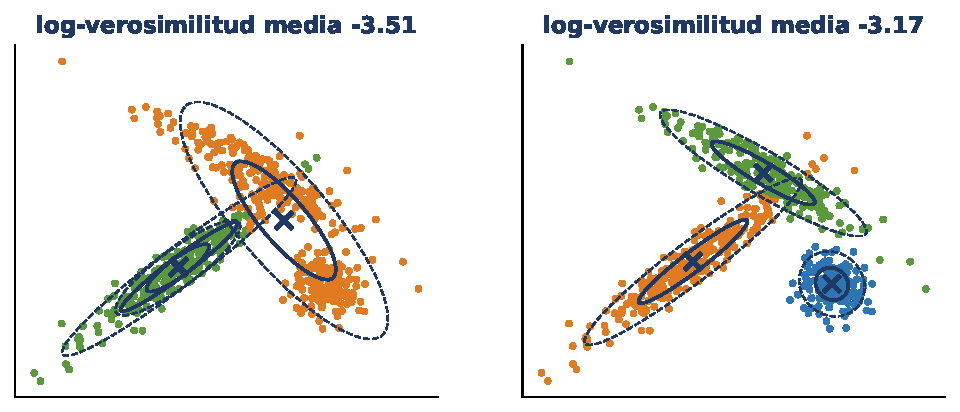
\includegraphics[width=\textwidth]{optimos_locales}
    \column{0.43\textwidth}
    \small
    \begin{itemize}
      \item Dos inicializaciones distintas sobre los mismos datos. La izquierda converge
            a un óptimo local (log-verosimilitud $-3.51$; ARI 0.49).
      \item Remedios en \texttt{GaussianMixture}:
        \begin{itemize}\scriptsize
          \item \texttt{n\_init}: varias corridas, se queda la de mayor verosimilitud;
          \item \texttt{init\_params="kmeans"} (por omisión): empieza desde k-medias.
        \end{itemize}
    \end{itemize}
  \end{columns}
  \vspace{6pt}
  \begin{alertblock}{Singularidades}
    Si un componente se queda con un solo punto, $|\Sig_k| \to 0$ y la verosimilitud crece
    sin límite. scikit-learn suma \texttt{reg\_covar} $=10^{-6}$ a la diagonal para evitarlo.
  \end{alertblock}
\end{frame}

\begin{frame}{k-medias como caso límite de EM}
  Fijemos $\Sig_k = \sigma^2 I$ y $\pi_k = 1/K$ para todo $k$. La responsabilidad queda
  \[
    \gamma_{ik} = \frac{\exp\!\big(-\|\x_i-\muv_k\|^2 / 2\sigma^2\big)}{\sum_j \exp\!\big(-\|\x_i-\muv_j\|^2 / 2\sigma^2\big)}
    \;\xrightarrow{\;\sigma \to 0\;}\;
    \begin{cases} 1 & \text{si } \muv_k \text{ es el centro más cercano}\\ 0 & \text{en otro caso}\end{cases}
  \]
  \begin{itemize}
    \item El paso E se vuelve la asignación al centro más cercano (paso de asignación de Lloyd).
    \item El paso M se vuelve el promedio de los puntos de cada grupo (paso de actualización).
  \end{itemize}
  \vspace{4pt}
  \begin{block}{Conclusión}
    k-medias es EM con grupos esféricos, iguales, y asignaciones duras.
    GMM relaja las tres restricciones.
  \end{block}
\end{frame}

% =====================================================================
\section{Tipos de matriz de covarianza}
% =====================================================================

\begin{frame}{Cuatro formas de restringir $\Sig_k$}
  \centering
  \renewcommand{\arraystretch}{1.25}
  \begin{tabular}{@{}llll@{}}
    \toprule
    \textbf{Tipo} & \textbf{Forma de $\Sig_k$} & \textbf{Grupos} & \textbf{Parámetros en $\Sig$}\\
    \midrule
    \texttt{"spherical"} & $\sigma_k^2 I$                 & esferas de radio propio      & $K$ \\
    \texttt{"diag"}      & $\operatorname{diag}(\sigma_{k1}^2,\dots,\sigma_{kd}^2)$ & elipses alineadas con los ejes & $Kd$ \\
    \texttt{"tied"}      & $\Sig$ (la misma para todos)   & elipses iguales              & $d(d+1)/2$ \\
    \texttt{"full"}      & $\Sig_k$ sin restricción       & elipses de cualquier forma   & $K\,d(d+1)/2$ \\
    \bottomrule
  \end{tabular}
  \vspace{8pt}
  \begin{itemize}
    \item A los de covarianza se suman $Kd$ parámetros de medias y $K-1$ de pesos.
    \item Ejemplo con $K=3$ y $d=4$ (Iris): \texttt{full} tiene $12 + 2 + 30 = 44$ parámetros;
          \texttt{spherical}, $12+2+3 = 17$.
    \item Con $d$ grande, \texttt{full} crece como $d^2$: más parámetros, más datos necesarios,
          más riesgo de sobreajuste.
  \end{itemize}
\end{frame}

\begin{frame}{Los cuatro tipos en el ejemplo detonador}
  \centering
  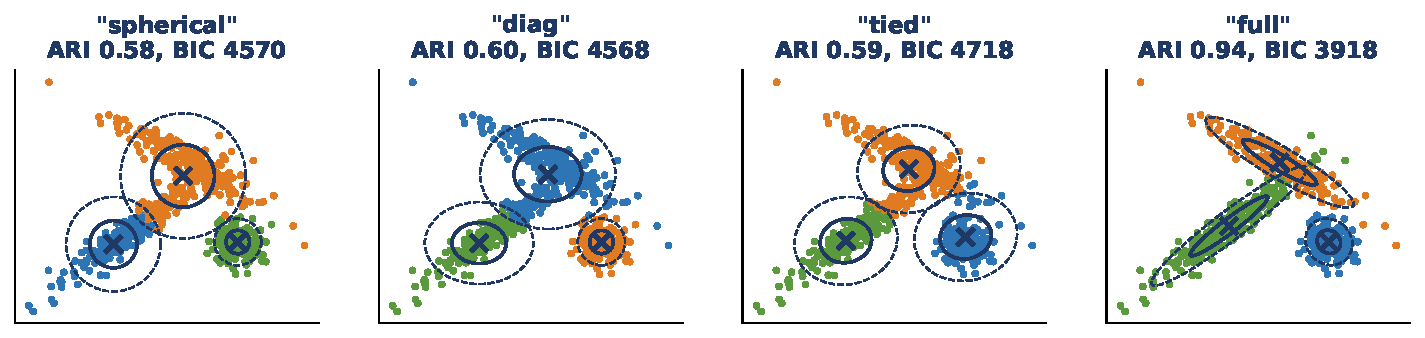
\includegraphics[width=\textwidth]{tipos_covarianza}
  \begin{itemize}
    \item \texttt{spherical} y \texttt{diag} no pueden inclinar las elipses; \texttt{tied}
          obliga a que los tres grupos tengan la misma forma.
    \item Sólo \texttt{full} recupera los grupos (ARI 0.94), y tiene el BIC más bajo
          a pesar de usar más parámetros.
  \end{itemize}
\end{frame}

% =====================================================================
\section{Selección de modelo con BIC y AIC}
% =====================================================================

\begin{frame}{Más componentes siempre ajustan mejor}
  \begin{itemize}
    \item La verosimilitud máxima nunca baja al agregar componentes o parámetros:
          no sirve para elegir $K$.
    \item Hay que penalizar la complejidad. Con $p$ parámetros libres y $n$ datos:
  \end{itemize}
  \[
    \text{AIC} = -2\,\ell(\hat\theta) + 2p
    \qquad\qquad
    \text{BIC} = -2\,\ell(\hat\theta) + p \log n
  \]
  \begin{columns}[T]
    \column{0.48\textwidth}
    \begin{block}{BIC (criterio bayesiano)}
      \begin{itemize}
        \item Penaliza más en cuanto $n \ge 8$ ($\log n > 2$).
        \item Consistente: con suficientes datos elige el modelo verdadero si está entre los candidatos.
        \item Tiende a elegir modelos simples.
      \end{itemize}
    \end{block}
    \column{0.48\textwidth}
    \begin{block}{AIC (criterio de Akaike)}
      \begin{itemize}
        \item Busca el mejor modelo para predecir datos nuevos.
        \item Con muestras grandes tiende a elegir más componentes.
        \item Más útil si el objetivo es estimar la densidad, no contar grupos.
      \end{itemize}
    \end{block}
  \end{columns}
  \vspace{4pt}
  {\small En los dos, \textbf{menor es mejor}. En scikit-learn: \texttt{gm.bic(X)} y \texttt{gm.aic(X)}.}
\end{frame}

\begin{frame}{Elegir $K$ y el tipo de covarianza}
  \begin{columns}[c]
    \column{0.5\textwidth}
    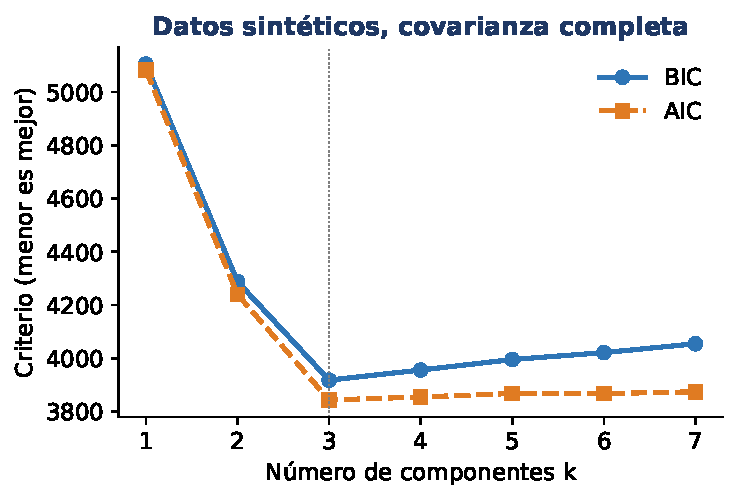
\includegraphics[width=\textwidth]{bic_sintetico}
    \column{0.48\textwidth}
    \small
    \begin{itemize}
      \item En el ejemplo detonador, BIC y AIC tienen su mínimo en $K=3$, el número de grupos
            con que se generaron los datos.
      \item Procedimiento: ajustar una rejilla de $K$ y de tipos de covarianza, y quedarse
            con el BIC más bajo.
      \item El BIC mide qué tan bien se describe la \textbf{densidad}; si los grupos no son
            gaussianos, puede pedir varios componentes para un solo grupo.
    \end{itemize}
  \end{columns}
\end{frame}

\begin{frame}[fragile]{Mezclas gaussianas en scikit-learn}
\begin{lstlisting}
from sklearn.mixture import GaussianMixture

gm = GaussianMixture(n_components=3,         # K
                     covariance_type="full",  # "full", "tied", "diag", "spherical"
                     n_init=10,               # corridas de EM; se queda la de mayor verosimilitud
                     random_state=0).fit(X)

gm.weights_, gm.means_, gm.covariances_      # parametros estimados
gm.converged_, gm.n_iter_                    # diagnostico de EM
etiquetas = gm.predict(X)                    # asignacion dura (argmax)
P = gm.predict_proba(X)                      # asignacion suave: n x K responsabilidades
gm.score_samples(X)                          # log p(x) de cada punto (densidad)
gm.bic(X), gm.aic(X)                         # seleccion de modelo
X_nuevos, z_nuevos = gm.sample(100)          # generar datos del modelo
\end{lstlisting}
  {\small \texttt{BayesianGaussianMixture} pone una distribución a priori sobre los pesos
  y puede apagar componentes que sobran.}
\end{frame}

% =====================================================================
%  Laboratorio (para omitirlo de las láminas, comentar la línea siguiente)
% =====================================================================
%  Laboratorio de la Sesión 4: GMM y k-medias en Iris
%  Se incluye desde Sesion4-GMM.tex con % =====================================================================
%  Laboratorio de la Sesión 4: GMM y k-medias en Iris
%  Se incluye desde Sesion4-GMM.tex con % =====================================================================
%  Laboratorio de la Sesión 4: GMM y k-medias en Iris
%  Se incluye desde Sesion4-GMM.tex con \input{Laboratorio}
%  El mismo código, ejecutado, está en laboratorio_gmm.ipynb
% =====================================================================
\section{Laboratorio: GMM y k-medias en Iris}
% =====================================================================

\begin{frame}[fragile]{Paso 1: ajustar la mezcla}
\begin{lstlisting}
import numpy as np, pandas as pd
from sklearn.datasets import load_iris
from sklearn.mixture import GaussianMixture
from sklearn.cluster import KMeans
from sklearn.metrics import adjusted_rand_score

X, especie = load_iris(return_X_y=True)     # la especie NO se usa para ajustar
gm = GaussianMixture(n_components=3, covariance_type="full", n_init=10, random_state=0).fit(X)
print(gm.converged_, gm.n_iter_, gm.weights_.round(2))
z = gm.predict(X)
print(pd.crosstab(z, especie), adjusted_rand_score(especie, z))
\end{lstlisting}
  \begin{columns}[T]
    \column{0.5\textwidth}
    \small
    \begin{itemize}
      \item EM converge en 17 iteraciones.
      \item Pesos: 0.30, 0.33 y 0.37.
      \item Índice de Rand ajustado contra la especie: \textbf{0.90}
            (k-medias obtuvo 0.73 en la Sesión 2).
    \end{itemize}
    \column{0.45\textwidth}
    \small
    \centering
    \begin{tabular}{@{}lccc@{}}
      & \textbf{setosa} & \textbf{versic.} & \textbf{virgin.}\\
      \midrule
      Comp. 1 & 0 & 45 & 0 \\
      Comp. 2 & 50 & 0 & 0 \\
      Comp. 3 & 0 & 5 & 50 \\
    \end{tabular}
  \end{columns}
\end{frame}

\begin{frame}[fragile]{Paso 2: asignaciones suaves}
\begin{lstlisting}
P = gm.predict_proba(X)                     # 150 x 3, cada fila suma 1
inciertas = np.where(P.max(axis=1) < 0.9)[0]
print((P.max(axis=1) > 0.99).sum(), inciertas, P[inciertas].round(2))
\end{lstlisting}
  \small
  \begin{itemize}
    \item 132 de las 150 flores tienen una probabilidad mayor que 0.99 en su componente.
    \item Sólo 3 tienen probabilidad máxima menor que 0.9:
  \end{itemize}
  \centering
  \begin{tabular}{@{}cccccc@{}}
    \toprule
    \textbf{Flor} & \textbf{Especie} & \textbf{Pétalo (cm)} & \textbf{P(comp. 1)} & \textbf{P(comp. 3)} & \textbf{Asignada a}\\
    \midrule
    77  & versicolor & $5.0 \times 1.7$ & 0.37 & 0.63 & comp. 3 (error) \\
    84  & versicolor & $4.5 \times 1.5$ & 0.86 & 0.14 & comp. 1 \\
    133 & virginica  & $5.1 \times 1.5$ & 0.24 & 0.76 & comp. 3 \\
    \bottomrule
  \end{tabular}
  \begin{itemize}
    \item Las tres están en la frontera entre versicolor y virginica: el modelo
          señala dónde puede equivocarse, cosa que k-medias no hace.
  \end{itemize}
\end{frame}

\begin{frame}[fragile]{Paso 3: comparar los tipos de covarianza}
\begin{lstlisting}
for tipo in ["full", "tied", "diag", "spherical"]:
    g = GaussianMixture(3, covariance_type=tipo, n_init=10, random_state=0).fit(X)
    z = g.predict(X)
    print(tipo, g._n_parameters(), round(g.bic(X), 1),
          round(adjusted_rand_score(especie, z), 2), np.bincount(z))
\end{lstlisting}
  \begin{columns}[c]
    \column{0.5\textwidth}
    \small
    \centering
    \begin{tabular}{@{}lccc@{}}
      \toprule
      \textbf{Tipo} & \textbf{Parám.} & \textbf{BIC} & \textbf{ARI}\\
      \midrule
      \texttt{full}      & 44 & 580.9 & 0.90 \\
      \texttt{tied}      & 24 & 633.8 & 0.89 \\
      \texttt{diag}      & 26 & 744.6 & 0.76 \\
      \texttt{spherical} & 17 & 853.8 & 0.73 \\
      \bottomrule
    \end{tabular}
    \column{0.48\textwidth}
    \small
    \begin{itemize}
      \item Los grupos de Iris son elipses inclinadas: las medidas de una flor están correlacionadas.
      \item \texttt{full} y \texttt{tied} las capturan.
      \item \texttt{spherical} obtiene el mismo ARI que k-medias (0.73).
      \item BIC ordena los tipos igual que el ARI, sin usar las especies.
    \end{itemize}
  \end{columns}
\end{frame}

\begin{frame}[fragile]{Paso 4: elegir $K$ con BIC y AIC}
\begin{lstlisting}
for tipo in ["full", "tied", "diag", "spherical"]:
    for k in range(1, 7):
        g = GaussianMixture(k, covariance_type=tipo, n_init=10, random_state=0).fit(X)
        print(tipo, k, round(g.bic(X), 1), round(g.aic(X), 1))
\end{lstlisting}
  \begin{columns}[c]
    \column{0.55\textwidth}
    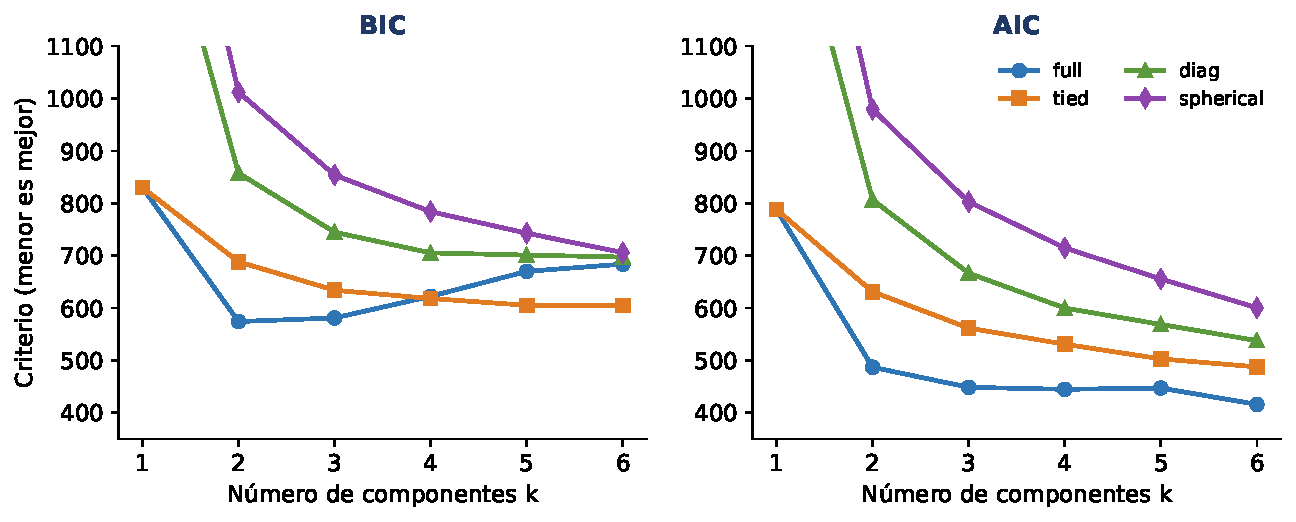
\includegraphics[width=\textwidth]{iris_bic}
    \column{0.43\textwidth}
    \small
    \begin{itemize}
      \item BIC más bajo: \texttt{full} con $K=2$ (574.0); $K=3$ queda muy cerca (580.9).
      \item Otra vez las dos escalas de Iris: setosa contra el resto, y después
            versicolor contra virginica.
      \item AIC sigue bajando con \texttt{full} hasta $K=6$ (415.7): penaliza menos y elige más
            componentes.
    \end{itemize}
  \end{columns}
\end{frame}

\begin{frame}[fragile]{Paso 5: GMM contra k-medias}
\begin{lstlisting}
z_km = KMeans(n_clusters=3, n_init=10, random_state=0).fit_predict(X)
print(pd.crosstab(z_km, especie), adjusted_rand_score(especie, z_km))
\end{lstlisting}
  \centering
  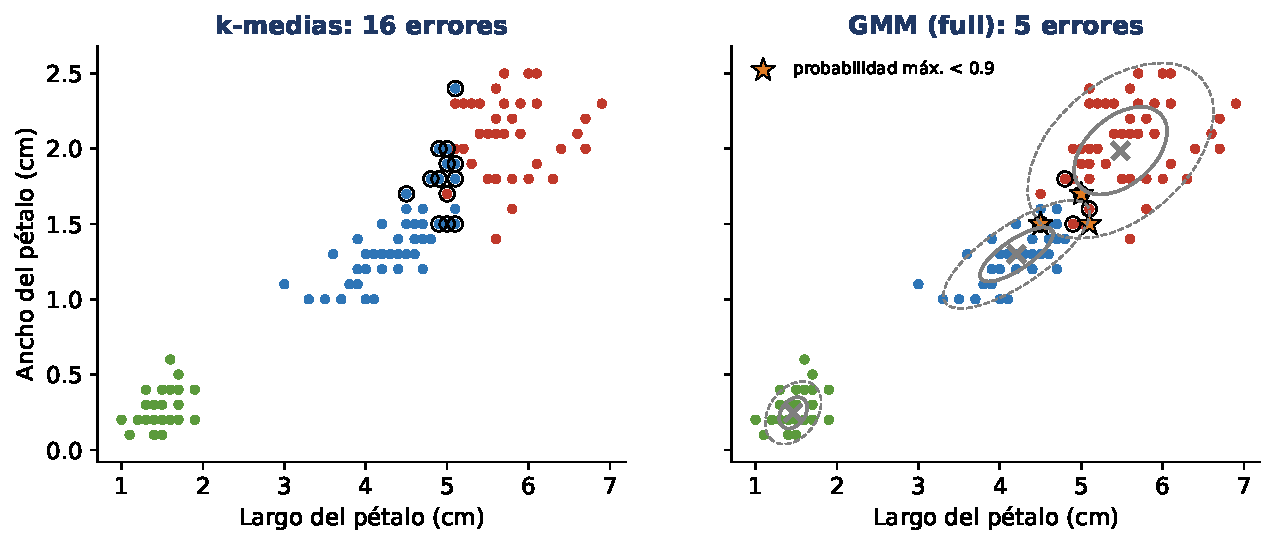
\includegraphics[width=0.66\textwidth]{iris_gmm}
  \small
  \begin{itemize}
    \item k-medias: 16 flores fuera de su especie (14 virginica con versicolor y 2 al revés);
          GMM: 5, todas versicolor. Círculos: errores; estrellas: flores inciertas.
    \item La elipse de virginica es más grande e inclinada; k-medias corta a la mitad entre los centros.
  \end{itemize}
\end{frame}

\begin{frame}{Conclusiones del laboratorio}
  \begin{itemize}
    \item Con covarianza completa, la mezcla gaussiana se acerca más a las especies que
          k-medias (ARI 0.90 contra 0.73) porque los grupos de Iris son elípticos.
    \item Las probabilidades indican qué flores están en la frontera; las 3 flores inciertas
          son de versicolor y virginica.
    \item El tipo de covarianza importa: \texttt{spherical} se comporta como k-medias.
    \item BIC elige el tipo de covarianza correcto sin usar etiquetas; para $K$ duda entre 2 y 3,
          igual que la silueta y el dendrograma en las sesiones anteriores.
    \item AIC elige demasiados componentes cuando el objetivo es contar grupos.
  \end{itemize}
\end{frame}

%  El mismo código, ejecutado, está en laboratorio_gmm.ipynb
% =====================================================================
\section{Laboratorio: GMM y k-medias en Iris}
% =====================================================================

\begin{frame}[fragile]{Paso 1: ajustar la mezcla}
\begin{lstlisting}
import numpy as np, pandas as pd
from sklearn.datasets import load_iris
from sklearn.mixture import GaussianMixture
from sklearn.cluster import KMeans
from sklearn.metrics import adjusted_rand_score

X, especie = load_iris(return_X_y=True)     # la especie NO se usa para ajustar
gm = GaussianMixture(n_components=3, covariance_type="full", n_init=10, random_state=0).fit(X)
print(gm.converged_, gm.n_iter_, gm.weights_.round(2))
z = gm.predict(X)
print(pd.crosstab(z, especie), adjusted_rand_score(especie, z))
\end{lstlisting}
  \begin{columns}[T]
    \column{0.5\textwidth}
    \small
    \begin{itemize}
      \item EM converge en 17 iteraciones.
      \item Pesos: 0.30, 0.33 y 0.37.
      \item Índice de Rand ajustado contra la especie: \textbf{0.90}
            (k-medias obtuvo 0.73 en la Sesión 2).
    \end{itemize}
    \column{0.45\textwidth}
    \small
    \centering
    \begin{tabular}{@{}lccc@{}}
      & \textbf{setosa} & \textbf{versic.} & \textbf{virgin.}\\
      \midrule
      Comp. 1 & 0 & 45 & 0 \\
      Comp. 2 & 50 & 0 & 0 \\
      Comp. 3 & 0 & 5 & 50 \\
    \end{tabular}
  \end{columns}
\end{frame}

\begin{frame}[fragile]{Paso 2: asignaciones suaves}
\begin{lstlisting}
P = gm.predict_proba(X)                     # 150 x 3, cada fila suma 1
inciertas = np.where(P.max(axis=1) < 0.9)[0]
print((P.max(axis=1) > 0.99).sum(), inciertas, P[inciertas].round(2))
\end{lstlisting}
  \small
  \begin{itemize}
    \item 132 de las 150 flores tienen una probabilidad mayor que 0.99 en su componente.
    \item Sólo 3 tienen probabilidad máxima menor que 0.9:
  \end{itemize}
  \centering
  \begin{tabular}{@{}cccccc@{}}
    \toprule
    \textbf{Flor} & \textbf{Especie} & \textbf{Pétalo (cm)} & \textbf{P(comp. 1)} & \textbf{P(comp. 3)} & \textbf{Asignada a}\\
    \midrule
    77  & versicolor & $5.0 \times 1.7$ & 0.37 & 0.63 & comp. 3 (error) \\
    84  & versicolor & $4.5 \times 1.5$ & 0.86 & 0.14 & comp. 1 \\
    133 & virginica  & $5.1 \times 1.5$ & 0.24 & 0.76 & comp. 3 \\
    \bottomrule
  \end{tabular}
  \begin{itemize}
    \item Las tres están en la frontera entre versicolor y virginica: el modelo
          señala dónde puede equivocarse, cosa que k-medias no hace.
  \end{itemize}
\end{frame}

\begin{frame}[fragile]{Paso 3: comparar los tipos de covarianza}
\begin{lstlisting}
for tipo in ["full", "tied", "diag", "spherical"]:
    g = GaussianMixture(3, covariance_type=tipo, n_init=10, random_state=0).fit(X)
    z = g.predict(X)
    print(tipo, g._n_parameters(), round(g.bic(X), 1),
          round(adjusted_rand_score(especie, z), 2), np.bincount(z))
\end{lstlisting}
  \begin{columns}[c]
    \column{0.5\textwidth}
    \small
    \centering
    \begin{tabular}{@{}lccc@{}}
      \toprule
      \textbf{Tipo} & \textbf{Parám.} & \textbf{BIC} & \textbf{ARI}\\
      \midrule
      \texttt{full}      & 44 & 580.9 & 0.90 \\
      \texttt{tied}      & 24 & 633.8 & 0.89 \\
      \texttt{diag}      & 26 & 744.6 & 0.76 \\
      \texttt{spherical} & 17 & 853.8 & 0.73 \\
      \bottomrule
    \end{tabular}
    \column{0.48\textwidth}
    \small
    \begin{itemize}
      \item Los grupos de Iris son elipses inclinadas: las medidas de una flor están correlacionadas.
      \item \texttt{full} y \texttt{tied} las capturan.
      \item \texttt{spherical} obtiene el mismo ARI que k-medias (0.73).
      \item BIC ordena los tipos igual que el ARI, sin usar las especies.
    \end{itemize}
  \end{columns}
\end{frame}

\begin{frame}[fragile]{Paso 4: elegir $K$ con BIC y AIC}
\begin{lstlisting}
for tipo in ["full", "tied", "diag", "spherical"]:
    for k in range(1, 7):
        g = GaussianMixture(k, covariance_type=tipo, n_init=10, random_state=0).fit(X)
        print(tipo, k, round(g.bic(X), 1), round(g.aic(X), 1))
\end{lstlisting}
  \begin{columns}[c]
    \column{0.55\textwidth}
    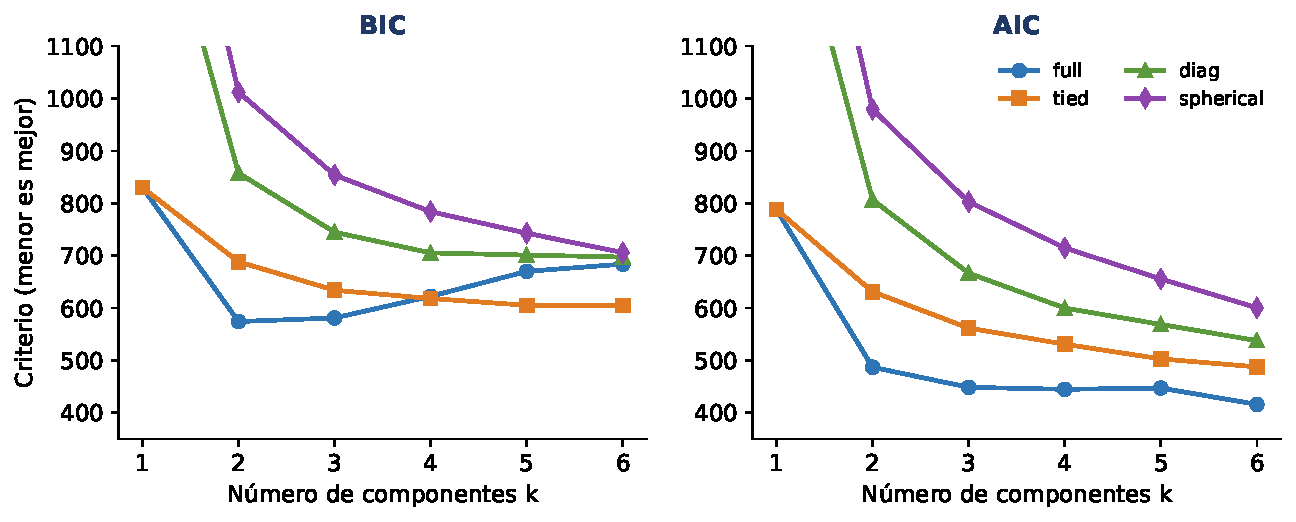
\includegraphics[width=\textwidth]{iris_bic}
    \column{0.43\textwidth}
    \small
    \begin{itemize}
      \item BIC más bajo: \texttt{full} con $K=2$ (574.0); $K=3$ queda muy cerca (580.9).
      \item Otra vez las dos escalas de Iris: setosa contra el resto, y después
            versicolor contra virginica.
      \item AIC sigue bajando con \texttt{full} hasta $K=6$ (415.7): penaliza menos y elige más
            componentes.
    \end{itemize}
  \end{columns}
\end{frame}

\begin{frame}[fragile]{Paso 5: GMM contra k-medias}
\begin{lstlisting}
z_km = KMeans(n_clusters=3, n_init=10, random_state=0).fit_predict(X)
print(pd.crosstab(z_km, especie), adjusted_rand_score(especie, z_km))
\end{lstlisting}
  \centering
  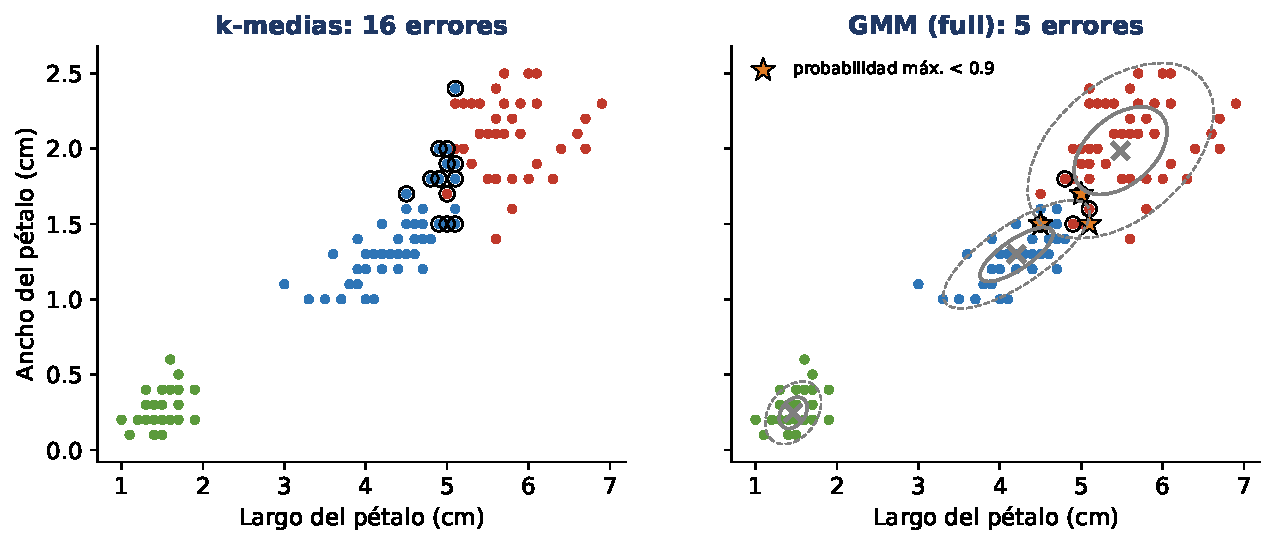
\includegraphics[width=0.66\textwidth]{iris_gmm}
  \small
  \begin{itemize}
    \item k-medias: 16 flores fuera de su especie (14 virginica con versicolor y 2 al revés);
          GMM: 5, todas versicolor. Círculos: errores; estrellas: flores inciertas.
    \item La elipse de virginica es más grande e inclinada; k-medias corta a la mitad entre los centros.
  \end{itemize}
\end{frame}

\begin{frame}{Conclusiones del laboratorio}
  \begin{itemize}
    \item Con covarianza completa, la mezcla gaussiana se acerca más a las especies que
          k-medias (ARI 0.90 contra 0.73) porque los grupos de Iris son elípticos.
    \item Las probabilidades indican qué flores están en la frontera; las 3 flores inciertas
          son de versicolor y virginica.
    \item El tipo de covarianza importa: \texttt{spherical} se comporta como k-medias.
    \item BIC elige el tipo de covarianza correcto sin usar etiquetas; para $K$ duda entre 2 y 3,
          igual que la silueta y el dendrograma en las sesiones anteriores.
    \item AIC elige demasiados componentes cuando el objetivo es contar grupos.
  \end{itemize}
\end{frame}

%  El mismo código, ejecutado, está en laboratorio_gmm.ipynb
% =====================================================================
\section{Laboratorio: GMM y k-medias en Iris}
% =====================================================================

\begin{frame}[fragile]{Paso 1: ajustar la mezcla}
\begin{lstlisting}
import numpy as np, pandas as pd
from sklearn.datasets import load_iris
from sklearn.mixture import GaussianMixture
from sklearn.cluster import KMeans
from sklearn.metrics import adjusted_rand_score

X, especie = load_iris(return_X_y=True)     # la especie NO se usa para ajustar
gm = GaussianMixture(n_components=3, covariance_type="full", n_init=10, random_state=0).fit(X)
print(gm.converged_, gm.n_iter_, gm.weights_.round(2))
z = gm.predict(X)
print(pd.crosstab(z, especie), adjusted_rand_score(especie, z))
\end{lstlisting}
  \begin{columns}[T]
    \column{0.5\textwidth}
    \small
    \begin{itemize}
      \item EM converge en 17 iteraciones.
      \item Pesos: 0.30, 0.33 y 0.37.
      \item Índice de Rand ajustado contra la especie: \textbf{0.90}
            (k-medias obtuvo 0.73 en la Sesión 2).
    \end{itemize}
    \column{0.45\textwidth}
    \small
    \centering
    \begin{tabular}{@{}lccc@{}}
      & \textbf{setosa} & \textbf{versic.} & \textbf{virgin.}\\
      \midrule
      Comp. 1 & 0 & 45 & 0 \\
      Comp. 2 & 50 & 0 & 0 \\
      Comp. 3 & 0 & 5 & 50 \\
    \end{tabular}
  \end{columns}
\end{frame}

\begin{frame}[fragile]{Paso 2: asignaciones suaves}
\begin{lstlisting}
P = gm.predict_proba(X)                     # 150 x 3, cada fila suma 1
inciertas = np.where(P.max(axis=1) < 0.9)[0]
print((P.max(axis=1) > 0.99).sum(), inciertas, P[inciertas].round(2))
\end{lstlisting}
  \small
  \begin{itemize}
    \item 132 de las 150 flores tienen una probabilidad mayor que 0.99 en su componente.
    \item Sólo 3 tienen probabilidad máxima menor que 0.9:
  \end{itemize}
  \centering
  \begin{tabular}{@{}cccccc@{}}
    \toprule
    \textbf{Flor} & \textbf{Especie} & \textbf{Pétalo (cm)} & \textbf{P(comp. 1)} & \textbf{P(comp. 3)} & \textbf{Asignada a}\\
    \midrule
    77  & versicolor & $5.0 \times 1.7$ & 0.37 & 0.63 & comp. 3 (error) \\
    84  & versicolor & $4.5 \times 1.5$ & 0.86 & 0.14 & comp. 1 \\
    133 & virginica  & $5.1 \times 1.5$ & 0.24 & 0.76 & comp. 3 \\
    \bottomrule
  \end{tabular}
  \begin{itemize}
    \item Las tres están en la frontera entre versicolor y virginica: el modelo
          señala dónde puede equivocarse, cosa que k-medias no hace.
  \end{itemize}
\end{frame}

\begin{frame}[fragile]{Paso 3: comparar los tipos de covarianza}
\begin{lstlisting}
for tipo in ["full", "tied", "diag", "spherical"]:
    g = GaussianMixture(3, covariance_type=tipo, n_init=10, random_state=0).fit(X)
    z = g.predict(X)
    print(tipo, g._n_parameters(), round(g.bic(X), 1),
          round(adjusted_rand_score(especie, z), 2), np.bincount(z))
\end{lstlisting}
  \begin{columns}[c]
    \column{0.5\textwidth}
    \small
    \centering
    \begin{tabular}{@{}lccc@{}}
      \toprule
      \textbf{Tipo} & \textbf{Parám.} & \textbf{BIC} & \textbf{ARI}\\
      \midrule
      \texttt{full}      & 44 & 580.9 & 0.90 \\
      \texttt{tied}      & 24 & 633.8 & 0.89 \\
      \texttt{diag}      & 26 & 744.6 & 0.76 \\
      \texttt{spherical} & 17 & 853.8 & 0.73 \\
      \bottomrule
    \end{tabular}
    \column{0.48\textwidth}
    \small
    \begin{itemize}
      \item Los grupos de Iris son elipses inclinadas: las medidas de una flor están correlacionadas.
      \item \texttt{full} y \texttt{tied} las capturan.
      \item \texttt{spherical} obtiene el mismo ARI que k-medias (0.73).
      \item BIC ordena los tipos igual que el ARI, sin usar las especies.
    \end{itemize}
  \end{columns}
\end{frame}

\begin{frame}[fragile]{Paso 4: elegir $K$ con BIC y AIC}
\begin{lstlisting}
for tipo in ["full", "tied", "diag", "spherical"]:
    for k in range(1, 7):
        g = GaussianMixture(k, covariance_type=tipo, n_init=10, random_state=0).fit(X)
        print(tipo, k, round(g.bic(X), 1), round(g.aic(X), 1))
\end{lstlisting}
  \begin{columns}[c]
    \column{0.55\textwidth}
    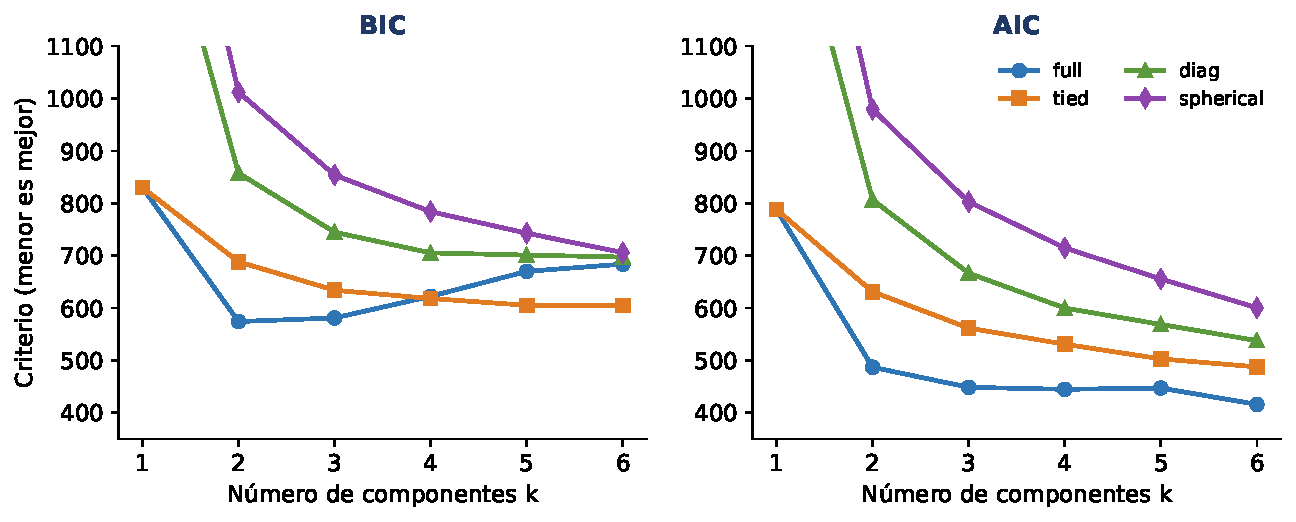
\includegraphics[width=\textwidth]{iris_bic}
    \column{0.43\textwidth}
    \small
    \begin{itemize}
      \item BIC más bajo: \texttt{full} con $K=2$ (574.0); $K=3$ queda muy cerca (580.9).
      \item Otra vez las dos escalas de Iris: setosa contra el resto, y después
            versicolor contra virginica.
      \item AIC sigue bajando con \texttt{full} hasta $K=6$ (415.7): penaliza menos y elige más
            componentes.
    \end{itemize}
  \end{columns}
\end{frame}

\begin{frame}[fragile]{Paso 5: GMM contra k-medias}
\begin{lstlisting}
z_km = KMeans(n_clusters=3, n_init=10, random_state=0).fit_predict(X)
print(pd.crosstab(z_km, especie), adjusted_rand_score(especie, z_km))
\end{lstlisting}
  \centering
  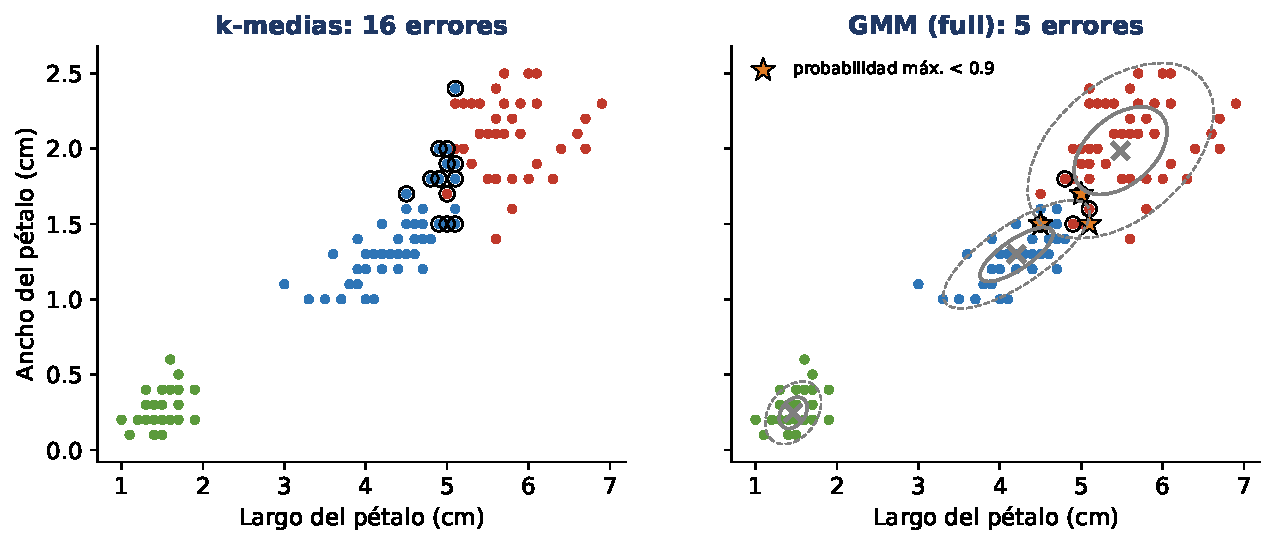
\includegraphics[width=0.66\textwidth]{iris_gmm}
  \small
  \begin{itemize}
    \item k-medias: 16 flores fuera de su especie (14 virginica con versicolor y 2 al revés);
          GMM: 5, todas versicolor. Círculos: errores; estrellas: flores inciertas.
    \item La elipse de virginica es más grande e inclinada; k-medias corta a la mitad entre los centros.
  \end{itemize}
\end{frame}

\begin{frame}{Conclusiones del laboratorio}
  \begin{itemize}
    \item Con covarianza completa, la mezcla gaussiana se acerca más a las especies que
          k-medias (ARI 0.90 contra 0.73) porque los grupos de Iris son elípticos.
    \item Las probabilidades indican qué flores están en la frontera; las 3 flores inciertas
          son de versicolor y virginica.
    \item El tipo de covarianza importa: \texttt{spherical} se comporta como k-medias.
    \item BIC elige el tipo de covarianza correcto sin usar etiquetas; para $K$ duda entre 2 y 3,
          igual que la silueta y el dendrograma en las sesiones anteriores.
    \item AIC elige demasiados componentes cuando el objetivo es contar grupos.
  \end{itemize}
\end{frame}

% =====================================================================

\begin{frame}{Resumen}
  \begin{itemize}
    \item Una mezcla gaussiana es un modelo generativo: cada grupo es una gaussiana con su
          peso, su media y su covarianza.
    \item Las responsabilidades $\gamma_{ik}$ dan asignaciones suaves y miden la incertidumbre.
    \item EM alterna el paso E (responsabilidades) y el paso M (parámetros); la verosimilitud
          nunca baja, pero converge a un máximo local.
    \item k-medias es el caso límite con covarianzas esféricas iguales y asignaciones duras.
    \item El tipo de covarianza controla la forma de los grupos y el número de parámetros.
    \item BIC y AIC penalizan la complejidad; BIC es el más usado para elegir $K$.
  \end{itemize}
  \vspace{6pt}
  \begin{block}{Próxima sesión}
    Agrupamiento por densidad y espectral: DBSCAN, HDBSCAN y grupos que no son convexos.
  \end{block}
\end{frame}

\end{document}
